% Drawing 45/03-1 -- folder 45, batch 03, archive page 52 (PDF page 53).
% Transcription: schéma d'implications sur deux rangées, que l'on résume : en haut « (iii') $\Leftrightarrow$ (i) $\Rightarrow$ (i') $\Leftrightarrow$ (ii) », suivi d'un « $\Leftrightarrow$ (iii') » biffé ; en bas « (iii) $\Leftrightarrow$ (i'') ». Entre les deux rangées, des flèches obliques dont plusieurs sont barrées en zigzag, deux portant « triviale » et une « \uncertain{inutile} » ; une grande courbe « triviale » joint (iii') à (iii). Des traits obliques renvoient aux lignes de droite : « \ill{} \uncertain{que} \uncertain{ce} \uncertain{ne} \uncertain{sont} \uncertain{pas} \uncertain{des} \uncertain{conditions} \ill{} », « \ill{} \uncertain{des} \ill{} \uncertain{du} \uncertain{nuage}\,? » et, biffé, « \uncertain{réalisations} de $T_1$ en $\Gamma_1$ \uncertain{et} $T_1$ »
% Kind: scheme of implications on two rows. Method 2 (schematic redraw from the facsimile). Status: partial.
% Notes: Upper row (iii') <=> (i) => (i') <=> (ii), lower row (iii) <=> (i''), labels at \small (drawing at 2 mm per crop unit, so that the labels keep the proportion of his writing). Between the rows the three arrows that are not struck, each a double arrow: (iii') region down to (iii), (i'') up to (i') with "triviale", up to (ii). "inutile" (uncertain in the transcription) is placed where it is written, between the struck arrows and the arrow marked "triviale". The large curve "triviale" starts under the heading Dem., runs down to the left of (iii') and passes just above (iii) to end at (i''), as on the facsimile. The reference lines: the curve from above (i) joining the upper line at the end of the row, the upper line, the lower line from (i''), and the four oblique lines, each starting on the upper line. Left out: the struck "<=> (iii')" after (ii), the two zigzag-struck arrows between (i) and (i') and their zigzags, the heading Dem., and the text on the right (it is in the transcription). Still differs: the lower line runs through the struck words "realisations de T_1 en Gamma_1 et T_1" and may be their strike-out rather than a reference line; it is kept, from (i'') to the end of those words. Redrawn 2026-11-09 (issue 128): to check again.
% Coordinates: 1 unit = 2 mm = 1/100 of the crop width (bbox in page fractions: [0.05, 0.4, 0.98, 0.6]).
% Redrawn by Claude (claude-opus-5-5), issue #73, 2026-11-09; not checked by a human; not compiled (no TeX in the session).
% Rights: reproduces part of the work -- behind RENDER_TRANSCRIPTS, never published by itself.
\documentclass[tikz,border=3pt]{standalone}
\usepackage{amsmath,amssymb}
\usetikzlibrary{patterns,arrows.meta}
\tikzset{pencil/.style={black!45}, struck/.style={black!35}, mark/.style={circle,draw,inner sep=1.3pt}, pt/.style={circle,fill,inner sep=0.9pt}, opt/.style={circle,draw,fill=white,inner sep=1.1pt}}
\begin{document}
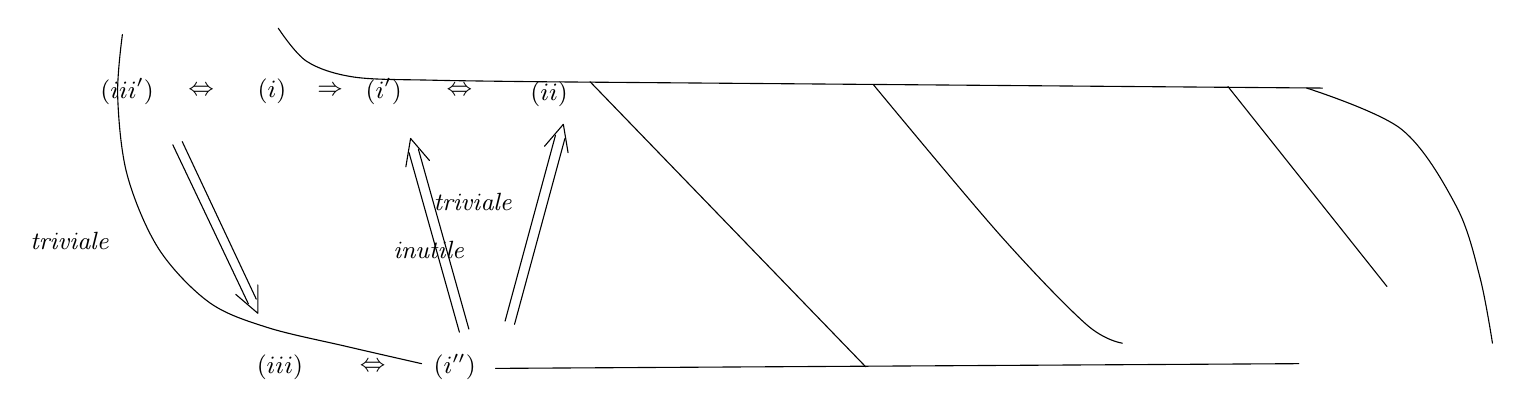
\begin{tikzpicture}[x=2mm,y=2mm,line cap=round,line join=round,font=\scriptsize]
\node[inner sep=1pt] at (10.6,-10.2) {\small $(iii')$};
\node[inner sep=1pt] at (15.3,-10.2) {\small $\Leftrightarrow$};
\node[inner sep=1pt] at (19.8,-10.2) {\small $(i)$};
\node[inner sep=1pt] at (23.5,-10.2) {\small $\Rightarrow$};
\node[inner sep=1pt] at (26.9,-10.2) {\small $(i')$};
\node[inner sep=1pt] at (31.7,-10.2) {\small $\Leftrightarrow$};
\node[inner sep=1pt] at (37.4,-10.4) {\small $(ii)$};
\node[inner sep=1pt] at (20.3,-27.7) {\small $(iii)$};
\node[inner sep=1pt] at (26.2,-27.7) {\small $\Leftrightarrow$};
\node[inner sep=1pt] at (31.4,-27.7) {\small $(i'')$};
\draw plot[smooth, tension=0.55] coordinates {(10.3,-6.6) (10,-10.5) (10.6,-15.5) (12.6,-20.2) (15.8,-23.6) (19.5,-25.2) (24.5,-26.4) (29.3,-27.5)};
\node[inner sep=1pt] at (7,-19.7) {\small \textit{triviale}};
\draw (13.5,-13.6) -- (18.3,-23.7);
\draw (14.1,-13.4) -- (18.8,-23.4);
\draw (18.9,-22.5) -- (18.9,-24.3) -- (17.5,-23.1);
\draw (32.3,-25.3) -- (29.1,-13.9);
\draw (31.7,-25.5) -- (28.5,-14.1);
\draw (28.3,-15) -- (28.6,-13.2) -- (29.8,-14.6);
\node[inner sep=1pt] at (32.6,-17.2) {\small \textit{triviale}};
\draw (35.2,-25) -- (38.4,-13.2);
\draw (34.6,-24.8) -- (37.8,-13);
\draw (37.1,-13.7) -- (38.3,-12.3) -- (38.6,-14.1);
\node[inner sep=1pt] at (29.8,-20.3) {\small \textit{inutile}};
\draw plot[smooth, tension=0.55] coordinates {(20.2,-6.2) (22,-8.3) (25,-9.3) (30,-9.5) (37,-9.6)};
\draw (37,-9.6) -- (86.5,-10);
\draw (34,-27.8) -- (85,-27.5);
\draw (40,-9.6) -- (57.5,-27.7);
\draw plot[smooth, tension=0.55] coordinates {(58,-9.8) (66,-19.3) (71.5,-25) (73.8,-26.2)};
\draw (80.5,-9.9) -- (90.6,-22.6);
\draw plot[smooth, tension=0.55] coordinates {(85.5,-10) (91.5,-12.6) (95,-17.5) (96.5,-22) (97.3,-26.2)};
\end{tikzpicture}
\end{document}
